\documentclass{standalone}
\usepackage{tikz}
\usepackage{ctex,siunitx}
\usepackage{tkz-euclide}
\usepackage{amsmath}
\usetikzlibrary{patterns, calc}
\usetikzlibrary {decorations.pathmorphing, decorations.pathreplacing, decorations.shapes,}
\begin{document}
\small
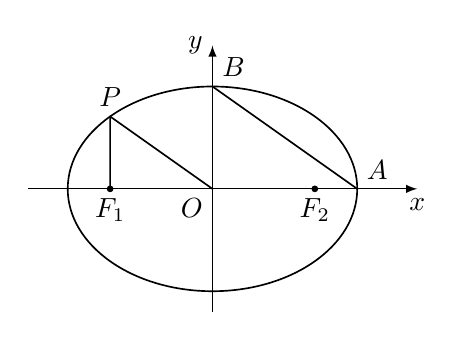
\begin{tikzpicture}[>=latex,scale=1.3]
  \tkzDefPoints{0/0/O,1.414/0/A,0/1/B,-1/0/F1,1/0/F2,-1/1/Fp}
  \tkzDefPointBy[translation=from A to B](O)\tkzGetPoint{A'}
  \tkzInterLL(F1,Fp)(O,A')\tkzGetPoint{P}
  \draw[thin,->](-1.8,0)--(2.0,0)node[below]{$x$};
  \draw[thin,->](0,-1.2)--(0,1.4)node[left]{$y$};
  \draw [semithick] (0,0) ellipse (1.414 and 1);
  \tkzDrawSegments[semithick](A,B P,O P,F1)
  \tkzDrawPoints[fill=black](F1,F2)
  \tkzLabelPoints[above right](A,B)
  \tkzLabelPoints[above](P)
  \tkzLabelPoints[below left](O)
  \tkzLabelPoint[below](F1){$F_1$}
  \tkzLabelPoint[below](F2){$F_2$}
\end{tikzpicture}
\end{document}